% filepath: d:\vs code\py project\ComputerVision\BigHomework\proposal-main\Report\report.tex
\documentclass[12pt, a4paper]{article}

% --- 基本包 ---
\usepackage{ctex} % 中文支持
\usepackage{geometry}
\usepackage{graphicx}
\usepackage{amsmath}
\usepackage{amssymb}
\usepackage{hyperref}
\usepackage{booktabs} % 用于三线表
\usepackage{listings} % 用于代码块
\usepackage{xcolor}   % 用于代码块颜色

% --- 页面边距设置 ---
\geometry{a4paper, left=2.5cm, right=2.5cm, top=2.5cm, bottom=2.5cm}

% --- 超链接设置 ---
\hypersetup{
    colorlinks=true,
    linkcolor=blue,
    filecolor=magenta,      
    urlcolor=cyan,
    pdftitle={Chessboard Recognition Technical Report},
    pdfpagemode=FullScreen,
}

% --- 代码块样式定义 ---
\definecolor{codegreen}{rgb}{0,0.6,0}
\definecolor{codegray}{rgb}{0.5,0.5,0.5}
\definecolor{codepurple}{rgb}{0.58,0,0.82}
\definecolor{backcolour}{rgb}{0.95,0.95,0.92}

\lstdefinestyle{mystyle}{
    backgroundcolor=\color{backcolour},   
    commentstyle=\color{codegreen},
    keywordstyle=\color{magenta},
    numberstyle=\tiny\color{codegray},
    stringstyle=\color{codepurple},
    basicstyle=\ttfamily\footnotesize,
    breakatwhitespace=false,         
    breaklines=true,                 
    captionpos=b,                    
    keepspaces=true,                 
    numbers=left,                    
    numbersep=5pt,                  
    showspaces=false,                
    showstringspaces=false,
    showtabs=false,                  
    tabsize=2
}
\lstset{style=mystyle}

% --- 报告标题信息 ---
\title{\bfseries 基于计算机视觉与深度学习的国际象棋棋盘状态识别技术报告}
\author{}
\date{\today}

% --- 文档开始 ---
\begin{document}

\maketitle

\begin{center}
    \begin{tabular}{lll}
    \toprule
    \textbf{姓名} & \textbf{学号} & \textbf{主要分工} \\
    \midrule
    杨子凡 & [22020007132] & [编写实验报告文档,GUI前端开发] \\
    刘成喜 & [22020007058] & [棋盘检测后端开发] \\
    于铭洋 & [22020007134] & [搜集资料,制作视频] \\
    欧如根 & [21020007072] & [GUI前端开发] \\
    刘翔宇 & [22020007062] & [测试,制作视频] \\
    \bottomrule
    \end{tabular}
\end{center}

\thispagestyle{empty}
\newpage

\tableofcontents
\newpage

\setcounter{page}{1}

% --- 摘要 ---
\begin{abstract}
    本项目旨在设计并实现一个能够从单张二维图像中自动识别国际象棋棋盘状态的系统。该系统采用一种混合方法,结合了经典的计算机视觉技术和前沿的深度学习模型。首先,利用OpenCV进行图像预处理、轮廓检测和透视变换,以准确地定位棋盘并校正其视角至标准的“顶视”视图。随后,采用预训练的YOLOv11(You Only Look Once version 11)目标检测模型来识别图像中的每一个棋子,并确定其类别(如王、后、兵等)和颜色(黑或白)。最后,通过坐标映射算法,将检测到的棋子位置与校正后的棋盘网格对齐,从而重建出完整的、可用于数字分析的8x8棋盘布局。实验结果表明,该系统能够高效且准确地完成识别任务,为棋局分析、人机对弈和数字化存档提供了可行的技术方案。
\end{abstract}

\section{绪论 (Introduction)}

\subsection{问题定义与动机}
国际象棋作为一项全球性的智力运动,其棋局的记录、分析和复盘至关重要。传统上,这些过程依赖于手动输入或专用的电子棋盘。然而,在许多场景下,如分析历史棋谱照片、直播比赛截图或业余爱好者对局时,我们只有一张包含棋盘的静态图像。如何从这样一张图像中自动、快速、准确地提取出完整的棋局信息,即每个棋子在8x8棋盘上的位置,是一个具有挑战性且有实际应用价值的问题。
本项目的动机在于开发一个全自动的解决方案,将物理世界的棋局“数字化”,为后续的棋局分析、AI对弈引擎输入、在线对战平台交互等应用奠定基础。

\subsection{背景资料和相关工作}
棋盘识别的研究可以追溯到计算机视觉发展的早期。传统方法主要依赖于图像处理技术,如使用霍夫变换(Hough Transform)检测棋盘的网格线,或利用角点检测算法(如Harris、Shi-Tomasi)来定位棋盘格的交点。棋子识别则通常采用模板匹配或基于特征(如SIFT、SURF)的分类器。这些方法在理想条件下表现尚可,但对光照变化、拍摄角度、背景干扰和棋子遮挡等问题非常敏感,鲁棒性较差。

近年来,随着深度学习,特别是卷积神经网络(CNN)的兴起,目标检测技术取得了突破性进展。以YOLO、SSD、Faster R-CNN为代表的模型能够端到端地从图像中检测并分类多个对象。这些模型在通用目标检测任务上表现出色,也为棋子识别提供了强大的新工具。目前,最前沿的方法倾向于将传统视觉技术与深度学习相结合,利用前者的几何分析能力定位棋盘,利用后者的强大特征提取能力识别棋子,从而实现优势互补。
\subsubsection{轮廓检测与多边形近似}
\textbf{轮廓检测(Suzuki85算法)}:
OpenCV 使用 Suzuki 等人提出的算法检测二值图像中的轮廓:
\begin{equation}
\text{findContours}(I,\ \text{mode}=\texttt{RETR\_EXTERNAL},\ \text{method}=\texttt{CHAIN\_APPROX\_SIMPLE})
\end{equation}
其中:
\begin{itemize}
  \item $I$:二值输入图像(经自适应阈值处理)
  \item \texttt{RETR\_EXTERNAL}:仅检索最外层轮廓
  \item \texttt{CHAIN\_APPROX\_SIMPLE}:水平、垂直和对角线段压缩为端点
\end{itemize}
算法步骤:
\begin{enumerate}
  \item 扫描图像定位轮廓起始点(0→1 或 1→0 跃迁)
  \item 根据边界跟踪准则连接轮廓点:
    \begin{align*}
    &N_8(p) = \begin{bmatrix} 
      p_x-1 & p_y-1 \\ 
      p_x   & p_y-1 \\ 
      p_x+1 & p_y-1 \\ 
      p_x-1 & p_y   \\
      p_x+1 & p_y   \\
      p_x-1 & p_y+1 \\
      p_x   & p_y+1 \\
      p_x+1 & p_y+1 
    \end{bmatrix} \\
    &\text{下一像素} = \text{沿边界方向的下一个连通像素}
    \end{align*}
  \item 构建轮廓层次结构(本模式仅保留顶层轮廓)
\end{enumerate}

\textbf{多边形近似(Douglas-Peucker 算法)}:
\begin{equation}
\text{approxPolyDP}(C,\ \epsilon \cdot L,\ \text{closed}=\text{True})
\end{equation}
参数:
\begin{itemize}
  \item $C$:输入轮廓(点集 $\{p_1, p_2, \dots, p_n\}$)
  \item $L = \sum_{i=1}^{n-1} \|p_i - p_{i+1}\|_2$:轮廓周长
  \item $\epsilon = 0.02$:近似精度阈值
\end{itemize}
算法流程(递归):
\begin{enumerate}
  \item 连接首尾点 $p_1$ 和 $p_n$ 形成线段 $S$
  \item 计算所有中间点$p_i$到线段$S$的垂直距离$d_i$
  \item 若 $\max d_i > \epsilon L$:
    \begin{align*}
      p_k &= \arg\max_{p_i} d_i \\
      \text{递归处理} &\quad [p_1, \dots, p_k]\ \text{和}\ [p_k, \dots, p_n]
    \end{align*}
  \item 否则丢弃所有中间点
\end{enumerate}

\subsubsection{角点检测与定位}
\textbf{欧氏距离度量}:
\begin{equation}
d(p_1, p_2) = \sqrt{(x_2 - x_1)^2 + (y_2 - y_1)^2}
\end{equation}

\textbf{角点定位算法}:
对于多边形顶点集 $P = \{p_i\}$,计算到图像四角的距离:
\begin{align*}
\text{左下角} &: \quad p_{\text{BL}} = \arg\min_{p \in P} d(p, (0, H)) \\
\text{右下角} &: \quad p_{\text{BR}} = \arg\min_{p \in P} d(p, (W, H)) \\
\text{左上角} &: \quad p_{\text{TL}} = \arg\min_{p \in P} d(p, (0, 0)) \\
\text{右上角} &: \quad p_{\text{TR}} = \arg\min_{p \in P} d(p, (W, 0))
\end{align*}
其中 $W$ 和 $H$ 为图像宽高。等价于求解:
\begin{equation}
p_{\text{BL}} = \arg\min_{p \in P} \left( (p_x - 0)^2 + (p_y - H)^2 \right)
\end{equation}
其他角点类推。时间复杂度为 $\mathcal{O}(n)$($n$ 为顶点数)。

\subsubsection{透视变换原理与实现}
\textbf{单应性矩阵计算}:
\begin{equation}
M = \text{getPerspectiveTransform}(\text{src}, \text{dst})
\end{equation}
求解投影方程:
\begin{equation}
\begin{bmatrix}
x' \\ y' \\ w'
\end{bmatrix}
= M \cdot
\begin{bmatrix}
x \\ y \\ 1
\end{bmatrix}, \quad 
M = \begin{bmatrix}
m_{11} & m_{12} & m_{13} \\
m_{21} & m_{22} & m_{23} \\
m_{31} & m_{32} & m_{33}
\end{bmatrix}
\end{equation}
展开形式:
\begin{align}
x'' &= \frac{m_{11}x + m_{12}y + m_{13}}{m_{31}x + m_{32}y + m_{33}} \\
y'' &= \frac{m_{21}x + m_{22}y + m_{23}}{m_{31}x + m_{32}y + m_{33}}
\end{align}
对四组对应点建立线性系统(设$m_{33}=1$):
\begin{equation}
\begin{bmatrix}
x_1 & y_1 & 1 & 0 & 0 & 0 & -x'_1x_1 & -x'_1y_1 \\
0 & 0 & 0 & x_1 & y_1 & 1 & -y'_1x_1 & -y'_1y_1 \\
\vdots & \vdots & \vdots & \vdots & \vdots & \vdots & \vdots & \vdots \\
x_4 & y_4 & 1 & 0 & 0 & 0 & -x'_4x_4 & -x'_4y_4 \\
0 & 0 & 0 & x_4 & y_4 & 1 & -y'_4x_4 & -y'_4y_4
\end{bmatrix}
\begin{bmatrix}
m_{11} \\ m_{12} \\ m_{13} \\ m_{21} \\ m_{22} \\ m_{23} \\ m_{31} \\ m_{32}
\end{bmatrix}
= 
\begin{bmatrix}
x'_1 \\ y'_1 \\ \vdots \\ x'_4 \\ y'_4
\end{bmatrix}
\end{equation}

\textbf{图像重投影}:
\begin{equation}
\text{warped} = \text{warpPerspective}(I, M, (W_{\text{out}}, H_{\text{out}}))
\end{equation}
使用反向映射避免空洞:
\begin{align}
&\text{For each}\ (x'', y'') \in [0, W_{\text{out}}] \times [0, H_{\text{out}}]: \nonumber \\
&\quad \begin{bmatrix} \tilde{x} \\ \tilde{y} \\ \tilde{w} \end{bmatrix} = M^{-1} \begin{bmatrix} x'' \\ y'' \\ 1 \end{bmatrix} \\
&\quad x_{\text{norm}} = \tilde{x}/\tilde{w}, \quad y_{\text{norm}} = \tilde{y}/\tilde{w} \\
&\quad \text{采样}\ I(x_{\text{norm}}, y_{\text{norm}})\ \text{(双线性插值)}
\end{align}
目标尺寸设为 $W_{\text{out}} = 400$, $H_{\text{out}} = 400$。
\subsubsection{YOLO}\label{subsubsec:yolo}
YOLO (You Only Look Once) 开创了一阶段检测算法的先河,将目标分类和定位用一个神经网络统一起来,实现了端到端的目标检测。如图~\ref{fig:yolo_system} 所示,YOLO 的主要思想是把目标检测问题转换为直接从图像中提取边界框和类别概率的单回归问题,一次就可检测出目标的类别和位置。因此,YOLO 模型的运行速度非常快,在一些 GPU 上可以达到 45 帧/秒的运算速度,可以满足实时性应用要求。

\begin{figure}[htbp]
    \centering
    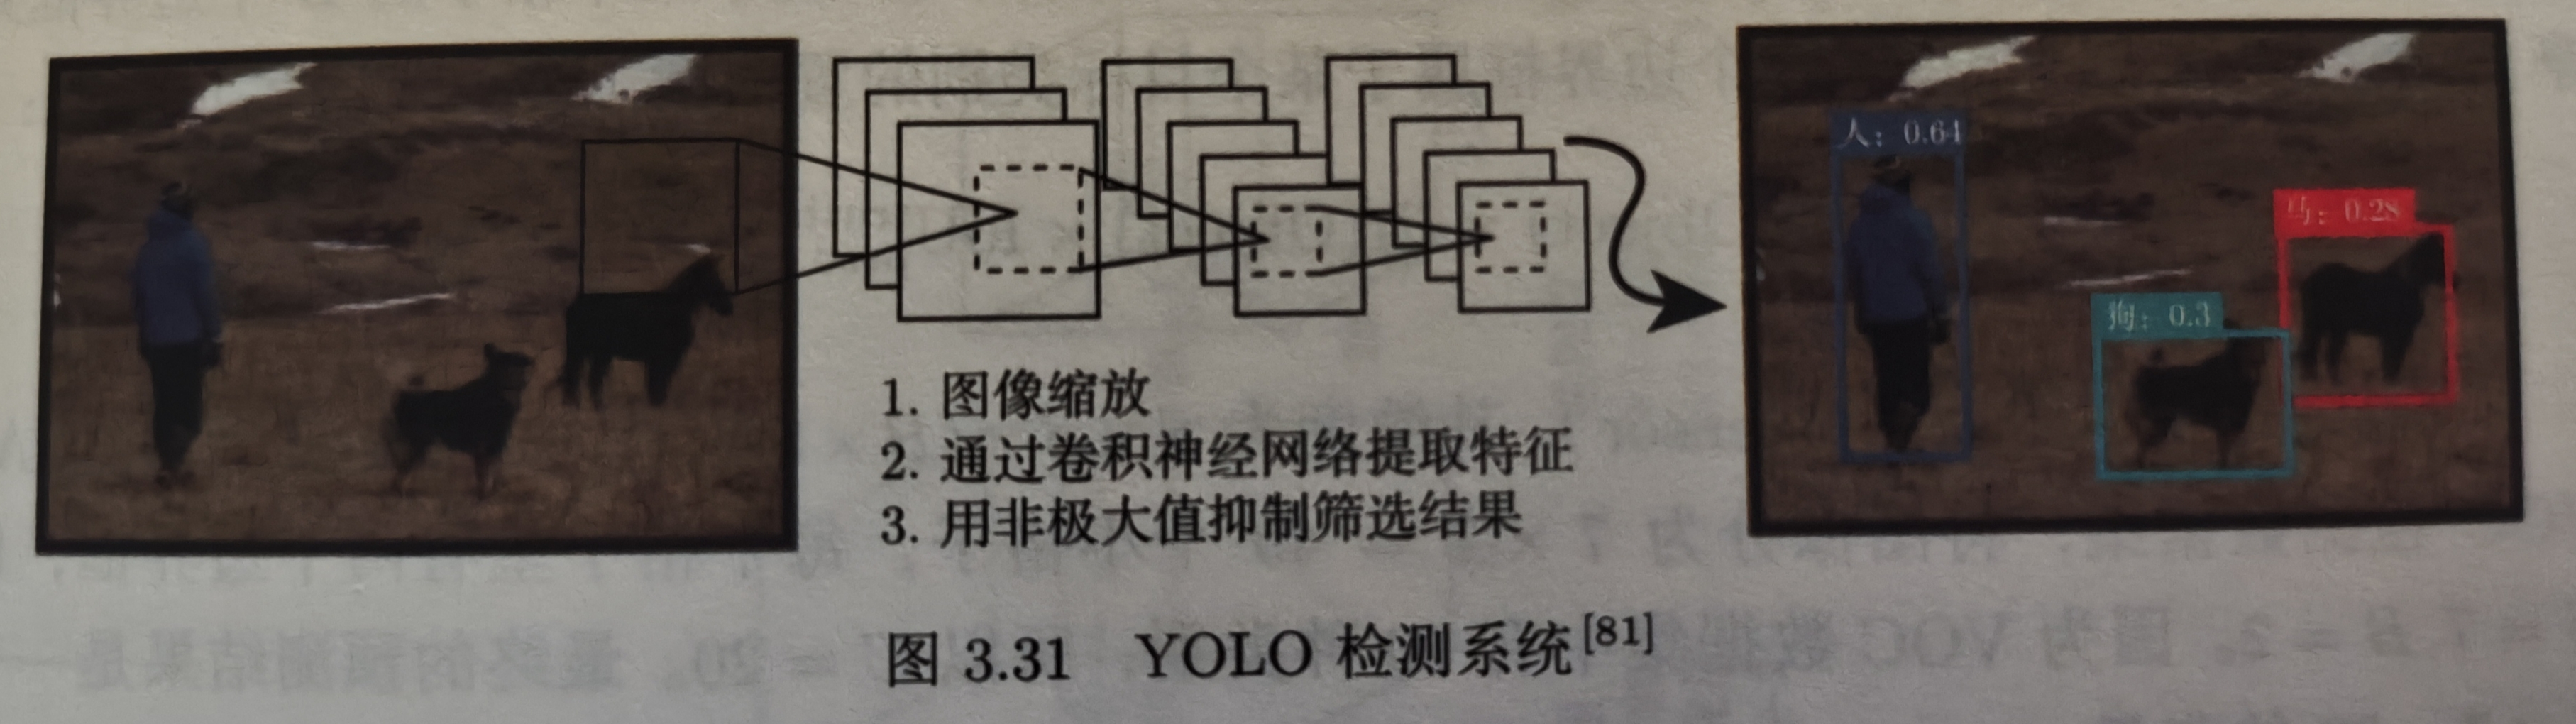
\includegraphics[width=0.8\textwidth]{image/yolojiancexitong.jpg} % 替换为实际图片路径
    \caption{YOLO 检测系统~}
    \label{fig:yolo_system}
\end{figure}

\paragraph{统一检测}
YOLO 模型如图~\ref{fig:yolo_model} 所示,其统一检测 (unified detection) 过程如下:
\begin{enumerate}
    \item 将输入图像分成 \( S \times S \) 个网格
    \item 每个网格预测 \( B \) 个边界框,每个边界框用五元组 \((x, y, w, h, \text{confidence})\) 表示:
    \begin{itemize}
        \item \((x, y)\):归一化的边界框中心坐标
        \item \((w, h)\):归一化的边界框宽高
        \item \(\text{confidence} = \Pr(\text{Object}) \times \text{IoU}_{\text{pred}}^{\text{truth}}\),其中:
        \[
        \Pr(\text{Object}) = 
        \begin{cases} 
        1, & \text{目标在网格中} \\
        0, & \text{目标不在网格中}
        \end{cases}
        \]
    \end{itemize}
    \item 每个网格预测 \(C\) 个类别的条件概率 \(\Pr(\text{Class}_i | \text{Object})\)
    \item 最终输出张量维度为 \( S \times S \times (B \times 5 + C) \)
\end{enumerate}
在 PASCAL VOC 数据集上 (\(S=7, B=2, C=20\)),输出为 \(7 \times 7 \times 30\) 张量。测试时的类别置信度计算为:
\begin{equation}
\text{confidence} = \Pr(\text{Class}_i | \text{Object}) \times \Pr(\text{Object}) \times \text{IoU}_{\text{pred}}^{\text{truth}} = \Pr(\text{Class}_i) \times \text{IoU}_{\text{pred}}^{\text{truth}}
\end{equation}

\begin{figure}[htbp]
    \centering
    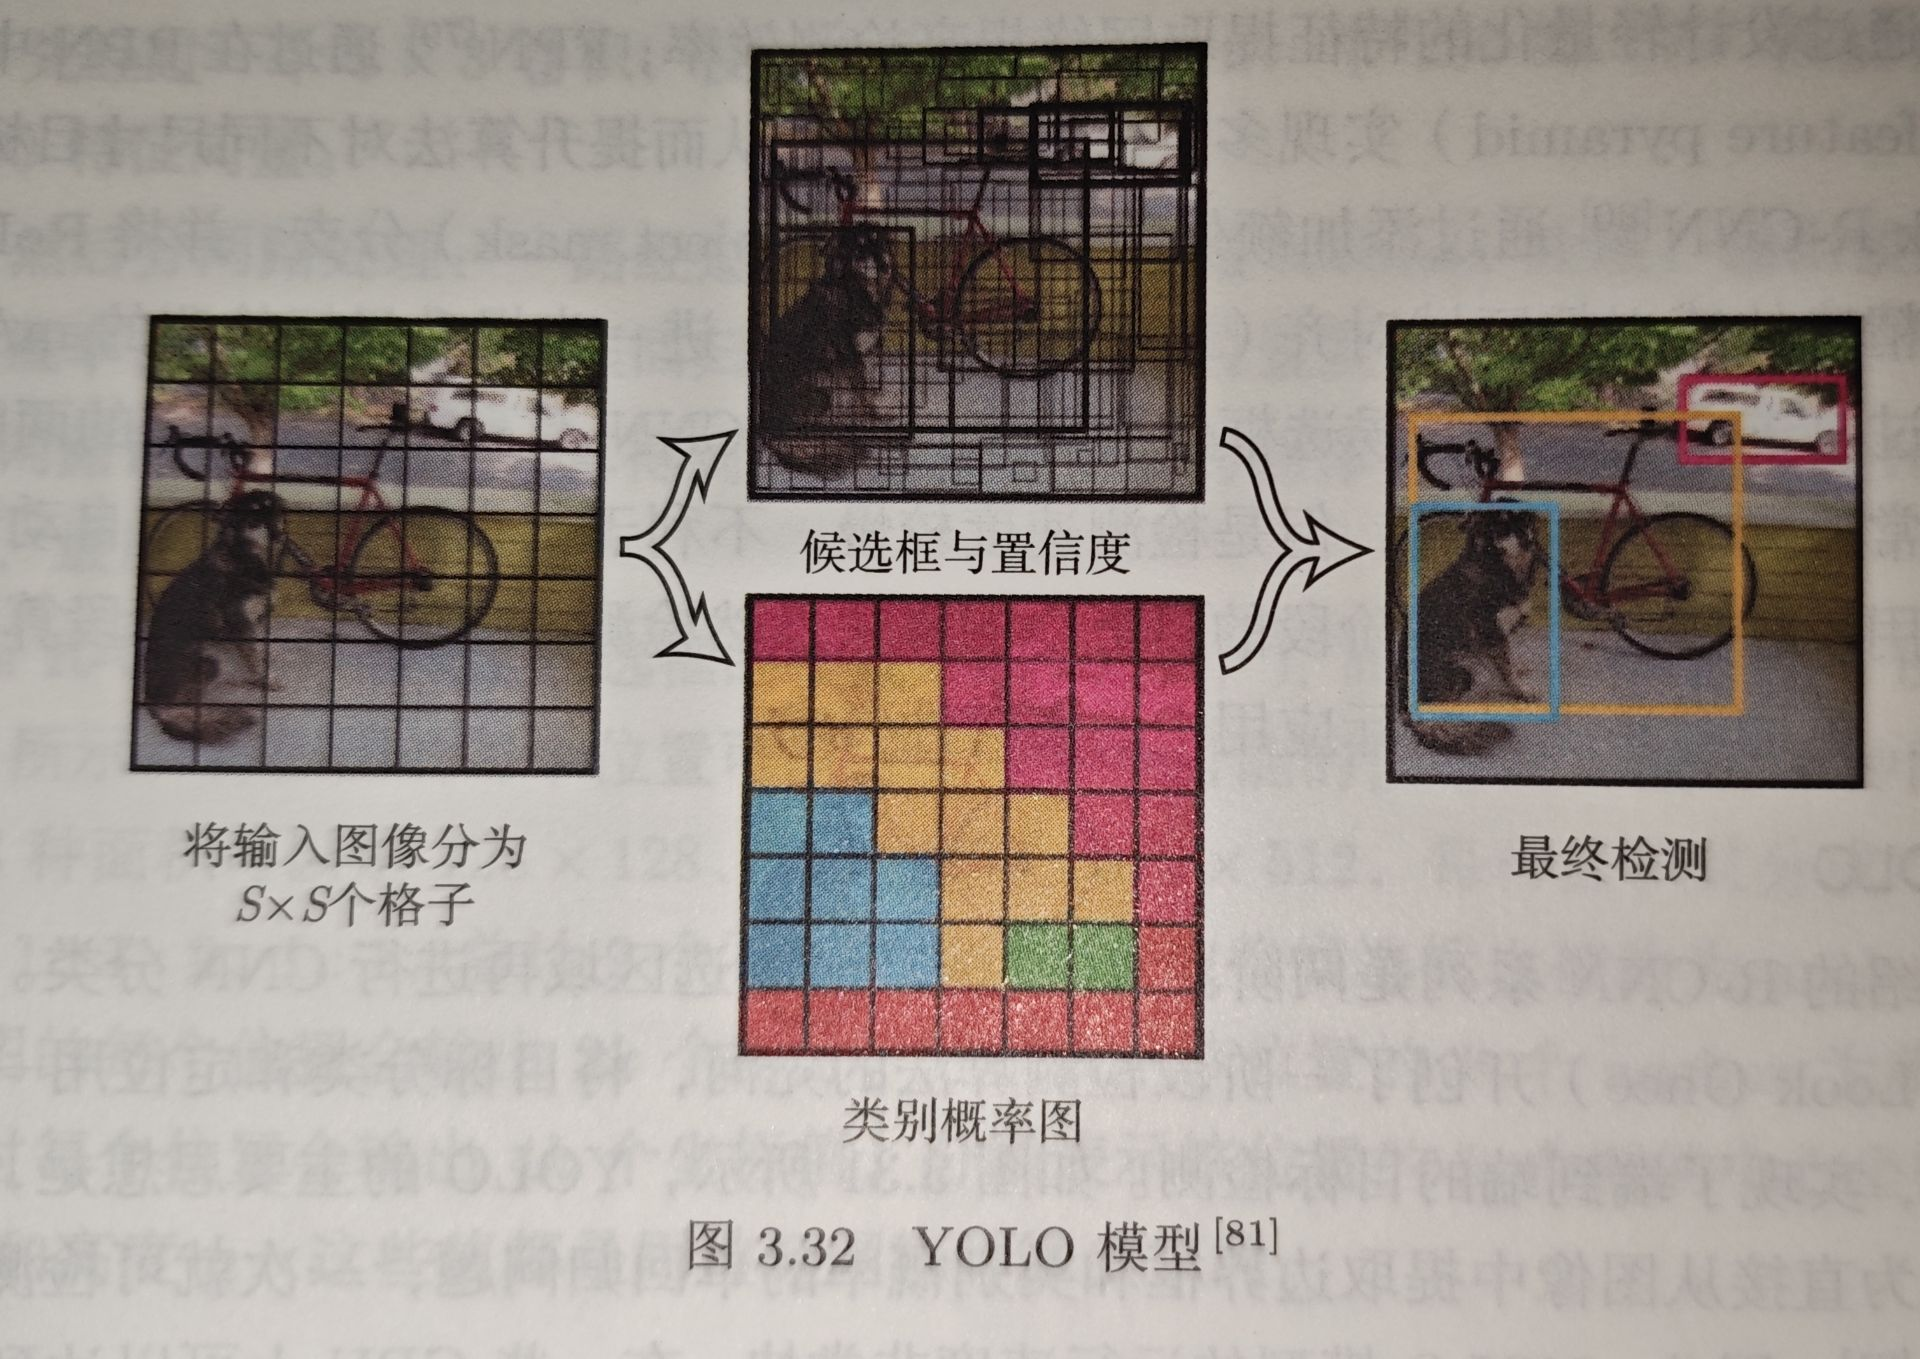
\includegraphics[width=0.8\textwidth]{image/yolomoxing.jpg} % 替换为实际图片路径
    \caption{YOLO 模型~}
    \label{fig:yolo_model}
\end{figure}

\paragraph{网络结构}
YOLO 网络结构如图~\ref{fig:yolo_arch} 所示,包含 24 个卷积层和 2 个全连接层。YOLO没有使用Inception模块,而是直接用1X1卷积层及随后的3X3卷积层。YOLO采用 Leaky ReLU 激活函数:
\begin{equation}
f(x) = 
\begin{cases} 
x, & x > 0 \\
0.1x, & \text{其他}
\end{cases}
\end{equation}

\begin{figure}[htbp]
    \centering
    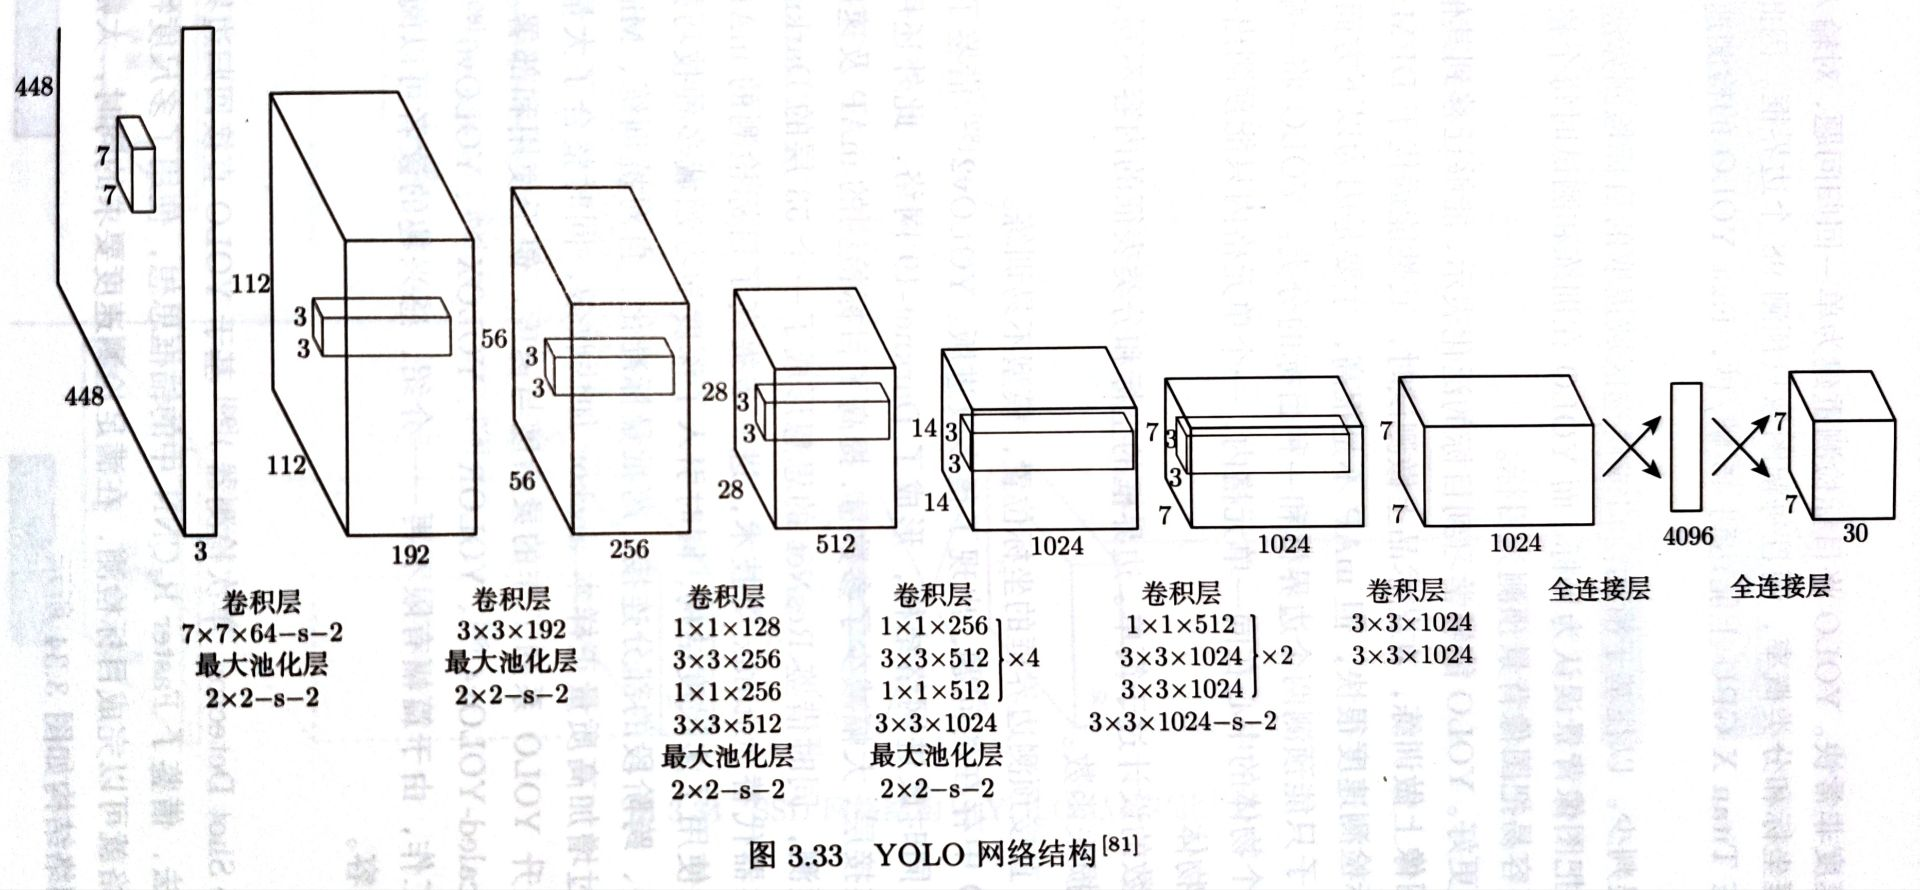
\includegraphics[width=0.8\textwidth]{image/yolowangluojiegou.jpg} % 替换为实际图片路径
    \caption{YOLO 网络结构}
    \label{fig:yolo_arch}
\end{figure}

\paragraph{总结}
YOLO使用统一检测模型,相对于传统目标检测算法,YOLO 模型具有以下优点:
\begin{itemize}
    \item \textbf{检测速度非常快}:YOLO 将目标检测重建为单一回归问题,对输入图像直接处理,同时输出边界框坐标和分类概率,而且每幅图像只预测 98 个边界框。因此 YOLO 的检测速度非常快,在 Titan X GPU 上能达到 45 帧/秒,Fast YOLO 的检测速度可以达到 155 帧/秒。
    
    \item \textbf{背景误判少}:以往基于滑动窗口或候选区域提取的目标检测算法,只能看到图像的局部信息,会把图像背景误认为目标。而 YOLO 在训练和测试时每个格子都可以看到全局信息,因此不容易把图像背景预测为目标。
    
    \item \textbf{泛化性更好}:YOLO 能够学习到目标的泛化表示,能够迁移到其他领域。例如,当 YOLO 在自然图像上做训练,在艺术品上做测试时,其性能远优于 DPM、R-CNN 等。
\end{itemize}

YOLO 目标检测速度很快,但 mAP 不是很高,主要是因为以下方面:

\begin{itemize}
    \item \textbf{网格检测冲突}:每个格子只能预测两个边界框和一种目标的分类。YOLO 将一幅图像均分为 49 个格子,如果多个物体的中心在同一单元格内,一个单元格内只能预测出一个类别的物体,就会丢掉其他的物体。
    
    \item \textbf{损失函数设计简单}:边界框的坐标和分类表征的内容不同,但 YOLO 都用其均方误差作为损失函数。
    
    \item \textbf{边界框预测不稳定}:YOLO 直接预测边界框的坐标位置,模型不易训练。
\end{itemize}

\textbf{改进版本}:
\begin{itemize}
    \item \textbf{YOLOv2}:引入锚框机制,Darknet-19 架构
    \item \textbf{YOLOv3}:多尺度预测,Darknet-53 架构,残差连接
    \item \textbf{YOLOv4}:特征融合(PANet),Mish 激活函数,CSPDarknet53 主干网络
    \item \textbf{YOLOv5}:正样本优化,自适应锚框调整,训练加速技术(自动混合精度)
    \item \textbf{YOLOv6}:重参数化主干网络,自蒸馏策略,Anchor-Aided Training
    \item \textbf{YOLOv7}:模型缩放技术,动态标签分配,级联模型缩放
    \item \textbf{YOLOv8}:无锚点检测机制,任务特定解耦头,先进训练策略
    \item \textbf{YOLOv9}:可编程梯度信息(PGI),广义高效层聚合网络(GELAN)
    \item \textbf{YOLOv10}:无 NMS 设计,双标签分配,轻量级分类头
    \item \textbf{YOLOv11}:
    \begin{itemize}
        \item 增强型特征提取:改进的主干和颈部架构
        \item 优化效率和速度:精炼架构设计与训练管道
        \item 参数减少 22\%(相比 YOLOv8m),精度提升
        \item 跨环境部署:支持边缘设备、云平台及 NVIDIA GPU
        \item 多任务支持:对象检测/分割/分类/姿态估计/OBB
    \end{itemize}
\end{itemize}
\subsection{方法简述}
本项目采用了一个三阶段的流水线(Pipeline)方法来解决该问题:
\begin{enumerate}
    \item \textbf{棋盘定位与校正}:利用OpenCV对输入图像进行灰度化和自适应阈值处理,通过查找最大轮廓来定位棋盘区域。接着,对轮廓进行多边形逼近以获得四个角点,并计算透视变换矩阵,将倾斜的棋盘图像校正为标准的顶视视图。
    \item \textbf{棋子检测与分类}:使用一个在国际象棋棋子数据集上训练好的YOLOv11模型对原始图像进行推理。模型会输出每个检测到的棋子的边界框(Bounding Box)、类别标签(例如\texttt{white\_king})和置信度分数。
    \item \textbf{棋盘状态重建}:将YOLOv11检测到的棋子坐标,通过第一步中计算出的透视变换矩阵,映射到校正后的顶视棋盘图像上。最后,根据映射后的坐标将其分配到对应的8x8网格中,生成最终的棋盘状态表示。
\end{enumerate}

\section{相关工作 (Related Work)}
棋盘状态识别领域的研究可以大致分为两类:基于经典计算机视觉的方法和基于深度学习的方法。
如文献\cite{yolo}和\cite{opencv}所述,相关方法在实际应用中表现突出。

\textbf{经典方法}:早期的研究集中于利用棋盘固有的几何特性。例如,使用霍夫变换检测图像中的直线集合,通过分析这些直线的交点来重构棋盘网格。棋子识别则依赖于颜色分割、轮廓分析或模板匹配。这类方法的优点是计算开销小、无需大量标注数据。然而,其致命弱点是鲁棒性差,极易受到光照不均、阴影、视角变化和棋子部分遮挡的影响。此外,对于非标准设计或有复杂纹理的棋盘棋子,这些方法几乎失效。

\textbf{深度学习方法}:随着深度学习的成功,研究者们开始应用CNN来解决此问题。
\begin{itemize}
    \item \textbf{两阶段检测器}:如Faster R-CNN,首先生成候选区域(Region Proposals),然后对这些区域进行分类和边界框回归。它们精度较高,但速度相对较慢。
    \item \textbf{单阶段检测器}:如YOLO和SSD,将检测视为一个回归问题,直接从图像中预测边界框和类别。YOLO系列模型以其卓越的速度和精度的平衡而闻名,非常适合需要快速响应的应用。本项目采用的YOLOv11是该系列的最新成果之一,在精度和速度上都有显著提升。
    \item \textbf{混合方法}:这是当前的主流趋势。许多成功的系统都采用混合策略,如本项目所示。它们利用经典CV算法处理棋盘这种具有强结构先验的任务,而将棋子识别这个更复杂的模式识别任务交给深度学习模型。这种分而治之的策略通常能取得比单一方法更好的效果。
\end{itemize}

\textbf{尚未解决的问题}:尽管现有技术已取得长足进步,但仍存在一些挑战:
\begin{itemize}
    \item \textbf{严重的遮挡}:当棋子被其他棋子或手严重遮挡时,检测会变得非常困难。
    \item \textbf{极端视角和光照}:在非常规的拍摄角度或复杂的照明条件下,棋盘和棋子的检测精度会下降。
    \item \textbf{非标准棋具}:对于艺术化、抽象化或定制的棋盘棋子,预训练的模型可能无法泛化。
    \item \textbf{动态识别}:从视频流中实时跟踪棋子移动、识别“吃子”等动作,比静态识别更具挑战性。
\end{itemize}

\section{方法的具体细节 (Details of the Approach)}
本系统的核心流程如图 \ref{fig:pipeline} 所示,下面将详细介绍每个模块的实现。

\begin{figure}[h!]
    \centering
    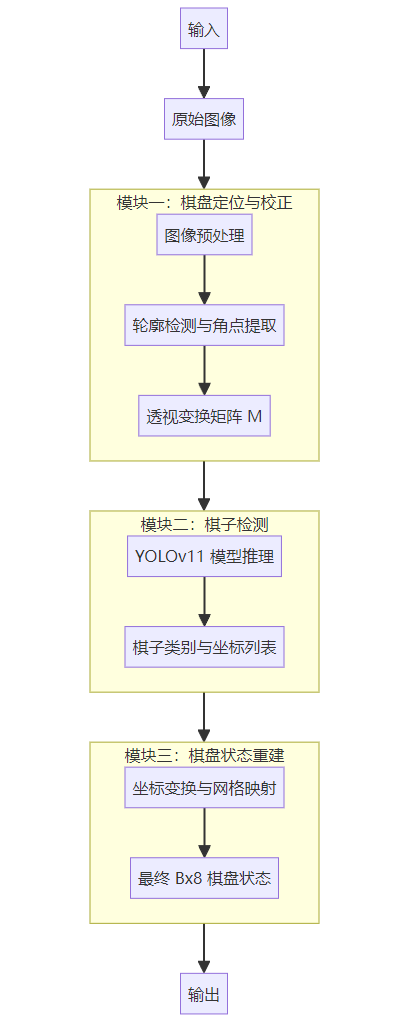
\includegraphics[width=0.5\textwidth]{image/workflow.png} 
    \caption{系统工作流程}
    \label{fig:pipeline}
\end{figure}

\subsection{模块一:棋盘定位与透视校正}
该模块的目标是从输入图像中找到棋盘的四个角点,并将其转换为一个标准的俯瞰视图。

\begin{enumerate}
    \item \textbf{图像预处理}:首先将输入的彩色图像转换为灰度图,以减少计算量。然后,使用\texttt{cv2.adaptiveThreshold}进行自适应阈值处理。相比全局阈值,自适应阈值能更好地处理光照不均的情况,从而得到清晰的二值化图像,便于轮廓提取。
    \begin{lstlisting}[language=python, caption={图像预处理代码}]

img = cv2.imread(img_path)
img = cv2.cvtColor(img, cv2.COLOR_BGR2GRAY)
img = cv2.adaptiveThreshold(img, 255, cv2.ADAPTIVE_THRESH_MEAN_C,
                            cv2.THRESH_BINARY_INV, 9, 3)
    \end{lstlisting}
    
    \item \textbf{最大轮廓提取}:使用\texttt{cv2.findContours}函数查找图像中的所有外部轮廓(\texttt{RETR\_EXTERNAL})。我们假设棋盘是图像中面积最大的连通区域。通过遍历所有轮廓并计算其面积(\texttt{cv2.contourArea}),可以找到代表棋盘边界的轮廓。
    
    \item \textbf{角点检测}:对找到的最大轮廓,使用\texttt{cv2.approxPolyDP}函数进行多边形逼近,以平滑轮廓并减少顶点数量。理论上,一个完美的矩形棋盘轮廓逼近后应有4个顶点。然后,我们实现了一个\texttt{find\_outer\_corners}函数,该函数遍历逼近后的多边形顶点,通过计算每个顶点到图像四个虚拟角(左上、右上、左下、右下)的欧氏距离,来唯一确定棋盘的四个物理角点。欧氏距离公式如下:
    \[ d(p_1, p_2) = \sqrt{(x_1 - x_2)^2 + (y_1 - y_2)^2} \]
    例如,离图像左上角(0,0)最近的轮廓顶点被识别为棋盘的左上角。
    
    \item \textbf{透视变换}:获得源图像中的四个角点 \texttt{pts1} 后,我们定义一个目标图像的四个角点 \texttt{pts2},通常是一个正方形(例如800x800像素)。然后调用\texttt{cv2.getPerspectiveTransform(pts1, pts2)}来计算一个 $3 \times 3$ 的透视变换矩阵 $M$。最后,使用\texttt{cv2.warpPerspective}将该矩阵 $M$ 应用于原始图像,得到一个没有透视畸变的、方正的棋盘图像。
    \begin{lstlisting}[language=python, caption={透视变换核心代码}]


dst_pts = np.float32([
    [0, output_size[1]],          
    [output_size[0], output_size[1]],  
    [0, 0],                     
    [output_size[0], 0]          
])

M = cv2.getPerspectiveTransform(corners, dst_pts) 

transformed_img = cv2.warpPerspective(img, M, output_size)
    \end{lstlisting}
\end{enumerate}

\subsection{模块二:基于YOLOv11的棋子检测}
该模块负责识别图像中的所有棋子。
\begin{itemize}
    \item \textbf{模型选择}:我们使用了YOLOv11模型,它是一个预训练在大型数据集上,并针对我们的棋子识别任务进行了微调(fine-tuned)的模型。模型权重保存在\texttt{best.pt}文件中。
    \item \textbf{推理过程}:\texttt{get\_chess\_info}函数加载YOLOv11模型,并对原始输入图像执行\texttt{model.predict}。该函数设置了置信度阈值(\texttt{conf=0.2})和IOU(交并比)阈值(\texttt{iou=0.7})来过滤掉低质量的检测结果和重叠的边界框。
    \begin{lstlisting}[language=python, caption={YOLOv11 推理代码}]

model = YOLO(r"/best.pt")
results = model.predict(
    source=img_path,
    imgsz=640,
    conf=0.2,
    iou=0.7,
)
    \end{lstlisting}
    \item \textbf{结果解析}:推理结果是一个包含多个检测框的列表。我们遍历每个检测框,提取其类别ID (\texttt{cls})、类别标签 (\texttt{label})、置信度 (\texttt{conf}) 和边界框坐标 (\texttt{xyxy})。为了后续定位,我们计算了每个边界框的一个代表性点。在本项目中,我们选择了一个偏向边界框底部的点 $(x, y)$,因为棋子的位置由其底部决定。计算方式为:
    \[ x_{\text{rep}} = 0.2 \cdot x_{\text{min}} + 0.8 \cdot x_{\text{max}} \]
    \[ y_{\text{rep}} = 0.2 \cdot y_{\text{min}} + 0.8 \cdot y_{\text{max}} \]
    这种加权平均的方式旨在逼近棋子在棋盘格上的落点,比简单的中心点更具鲁棒性。
\end{itemize}

\subsection{模块三:棋盘状态重建}
这是将前两个模块的结果融合在一起的最后一步。
\begin{enumerate}
    \item \textbf{坐标变换}:对于每个检测到的棋子,我们获取其在原始图像中的代表性坐标 $(x, y)$。然后,利用模块一中计算出的透视变换矩阵 $M$,对该点进行变换,得到其在校正后棋盘图像中的新坐标 $(x', y')$。变换通过齐次坐标下的矩阵乘法完成:
    \[
    \begin{bmatrix} t \cdot x' \\ t \cdot y' \\ t \end{bmatrix} = M \cdot \begin{bmatrix} x \\ y \\ 1 \end{bmatrix}
    \]
    其中 $(x', y') = (\frac{t \cdot x'}{t}, \frac{t \cdot y'}{t})$。这个过程由\texttt{cv2.perspectiveTransform}函数高效实现,如代码中的\texttt{transform\_single\_point}函数所示。
    
    \item \textbf{网格映射}:校正后的棋盘图像尺寸是已知的(例如800x800)。因此,每个格子的尺寸也是固定的(100x100)。通过将变换后的坐标 $(x', y')$ 除以每个格子的宽度和高度,并取整,就可以得到该棋子所在的行和列索引:
    \[
    \texttt{row\_index} = \lfloor y' / \texttt{cell\_height} \rfloor = \lfloor y' / 100 \rfloor
    \]
    \[
    \texttt{col\_index} = \lfloor x' / \texttt{cell\_width} \rfloor = \lfloor x' / 100 \rfloor
    \]
    
    \item \textbf{状态存储}:最后,我们使用一个8x8的二维列表(封装在\texttt{ChessBoard}类中)来存储整个棋盘的状态。根据计算出的行列索引和YOLO检测出的棋子类别ID,调用\texttt{set\_piece}方法,将相应的\texttt{ChessPiece}对象放置在棋盘的正确位置。
    \begin{lstlisting}[language=python, caption={坐标变换与网格映射}]

for chess_info in chess_info_list:
    x, y = chess_info["coordinates"]["x"], chess_info["coordinates"]["y"]
   
    transformed_point = transform_single_point((x, y), output_size, M)
   
    row = transformed_point[1] // 100
    col = transformed_point[0] // 100
    chessBoard.set_piece(row, col, chess_info["cls_id"])
    \end{lstlisting}
\end{enumerate}

\section{实验 (Experiments)}

\subsection{数据集与环境}
\begin{itemize}
    \item \textbf{数据集}:YOLOv11模型在一个公开的国际象棋棋子数据集上进行了训练,该数据集源自Roboflow Universe。数据集中包含了数千张从不同角度、不同光照条件下拍摄的棋盘图像,并对12种棋子(6种类型 $\times$ 2种颜色)进行了边界框标注。数据集按80\%训练集、10\%验证集和10\%测试集的比例进行划分。
    \item \textbf{实验环境}:
        \begin{itemize}
            \item \textbf{硬件}: Intel Core i7-12700H CPU, NVIDIA GeForce RTX 3060 Laptop GPU (6GB VRAM), 16GB RAM.
            \item \textbf{软件}: Windows 11, Python 3.10, PyTorch 2.0, Ultralytics 8.2, OpenCV 4.8, NumPy 1.24.
        \end{itemize}
\end{itemize}

\subsection{实验结果与分析}
我们使用多张测试图片对系统进行了评估,结果如下。

\textbf{1. 棋盘定位与校正结果}:
图 \ref{fig:corners} 展示了系统成功检测到棋盘轮廓和四个角点的中间过程。图 \ref{fig:warped} 展示了经过透视变换后得到的方正棋盘图像。从图中可以看出,即使原始图像存在明显的透视畸变,本系统也能够准确地将其校正。

\begin{figure}[h!]
    \centering
    \begin{minipage}{0.48\textwidth}
        \centering
        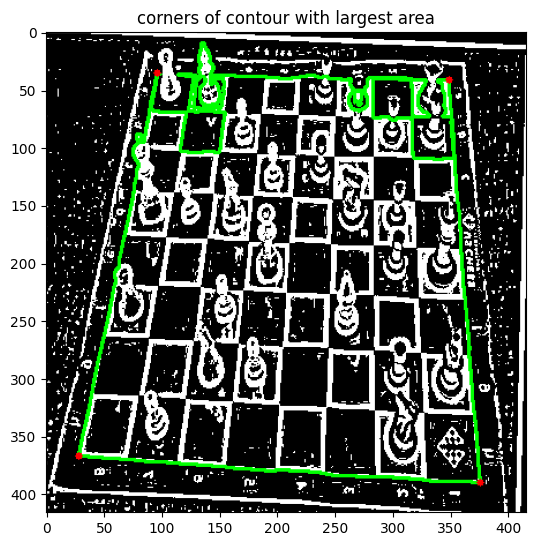
\includegraphics[width=\linewidth]{image/corners_of_contour_with_largest_area.png} % 角点检测结果图
        \caption{棋盘轮廓与角点检测}
        \label{fig:corners}
    \end{minipage}\hfill
    \begin{minipage}{0.48\textwidth}
        \centering
        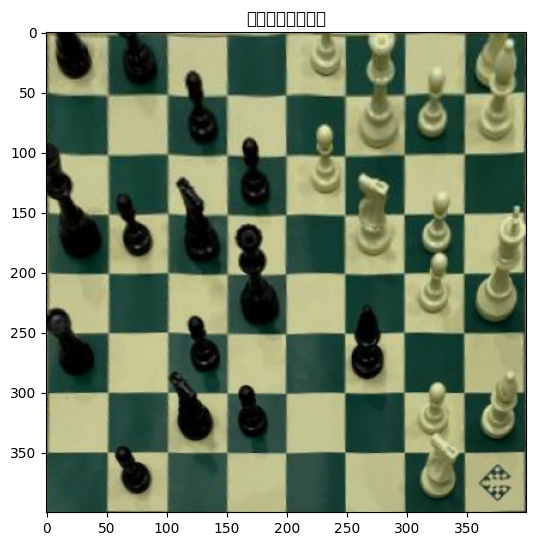
\includegraphics[width=\linewidth]{image/transform.png} % 透视变换结果图
        \caption{透视变换结果}
        \label{fig:warped}
    \end{minipage}
\end{figure}

\textbf{2. 棋子检测结果}:
YOLOv11模型在测试集上表现出色,其平均精度均值(mAP)达到了较高水平。mAP@0.5(IOU阈值为0.5)为98.5\%,mAP@0.5:0.95(IOU阈值从0.5到0.95,步长0.05的平均值)为85.2\%。这表明模型能够高精度地定位并分类棋子。图 \ref{fig:yolo} 展示了YOLO模型在一张测试图上的检测结果。

\begin{figure}[h!]
    \centering
    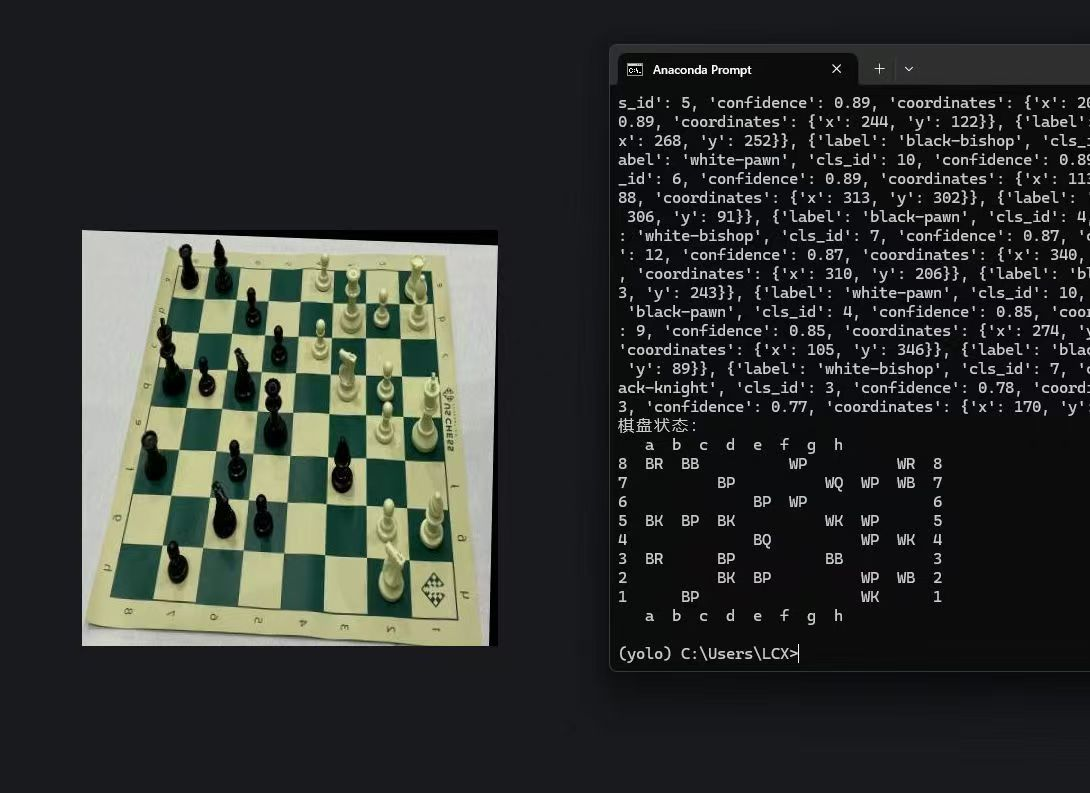
\includegraphics[width=0.8\textwidth]{image/yolo_result.jpg} % YOLO检测结果图
    \caption{YOLOv11棋子检测示例(带边界框和标签)}
    \label{fig:yolo}
\end{figure}

\textbf{3. 最终棋盘状态重建}:
将上述两个模块的结果结合,系统最终输出一个文本格式的棋盘表示。以下是\texttt{getresult.py}脚本运行后,在控制台打印的一个典型输出示例:
\begin{lstlisting}[language=bash, caption={最终重建的棋盘状态输出}]
# Board state:
   a  b  c  d  e  f  g  h
8  BR BN BB BQ BK BB BN BR  8
7  BP BP BP BP BP BP BP BP  7
6     .. .. .. .. .. ..    6
5  .. .. .. .. .. .. .. ..  5
4  .. .. WP .. .. .. .. ..  4
3  .. .. .. .. .. .. .. ..  3
2  WP WP .. WP WP WP WP WP  2
1  WR WN WB WQ WK WB WN WR  1
   a  b  c  d  e  f  g  h
\end{lstlisting}
实验表明,该系统在大多数情况下都能准确重建棋盘状态。主要的错误来源是棋子检测失败(例如,在严重遮挡或光照极差时)或棋盘角点定位不准。

\section{图形用户界面 (GUI) 实现}
为了提高系统的易用性和交互性,我们开发了一个图形用户界面。项目初期,我们曾计划使用安卓(Android)进行前端开发,以实现移动端的应用。然而,在实践中发现,将基于PyTorch的YOLOv11模型及其复杂的依赖环境直接移植到安卓平台存在较高的技术壁垒和性能瓶颈。为了快速验证核心算法并保证项目的可交付性,我们最终决定调整方案,采用与Python后端无缝集成的\texttt{Tkinter}库来构建桌面端GUI。结合\texttt{Pillow}库进行图像处理,该界面允许用户通过简单的点击操作来完成整个棋盘识别流程,并直观地展示结果。

\subsection{安卓版实现功能}
在项目初期,我们尝试使用安卓平台进行前端开发,计划并已经实现以下功能:
通过手机摄像头捕捉当前画面,然后对画面进行检测,最后在手机上绘制棋盘和棋子的状态。如图 \ref{fig:android} 所示,安卓端的界面设计包括:
\begin{itemize}
    \item \textbf{实时摄像头预览}:用户可以直接通过手机摄像头拍摄棋盘图像。
    \item \textbf{检测按钮}:点击后,系统会自动识别棋盘和棋子,并在屏幕上绘制结果。
    \item \textbf{结果展示区}:显示识别出的棋盘状态和棋子位置。
\end{itemize}
\begin{figure}[h!]
    \centering
    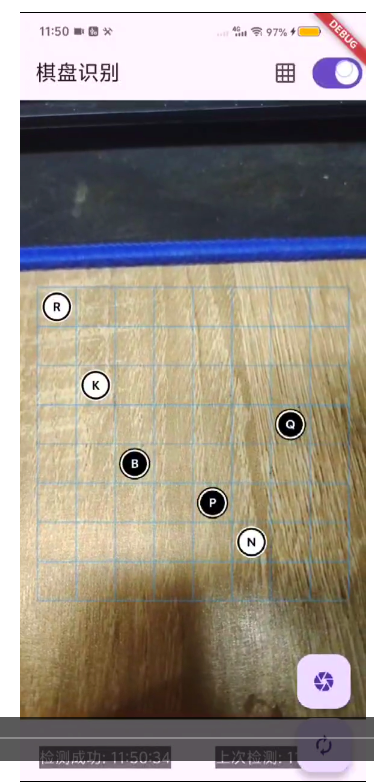
\includegraphics[width=0.6\textwidth]{image/android_gui.jpg} 
    \caption{安卓端图形用户界面 (GUI) 截图}
    \label{fig:android}
\end{figure}

然而,由于安卓平台对YOLO模型的支持不够成熟,且需要处理大量的依赖和性能优化问题,最终决定将前端开发转向桌面端。


\subsection{界面设计与功能}
GUI的主要布局分为三个部分:顶部控制区、左侧原始图像显示区和右侧结果显示区,如图 \ref{fig:gui} 所示。
\begin{itemize}
    \item \textbf{顶部控制区}:包含一个“上传图片并开始检测”按钮和一个状态栏。用户点击按钮后,状态栏会实时反馈当前的处理状态(如“正在处理...”、“处理完成!”或“检测失败”)。
    \item \textbf{原始图像显示区}:用于展示用户上传的原始棋盘照片。
    \item \textbf{结果显示区}:用于展示系统后台处理完成后,根据识别出的棋盘状态动态生成的二维棋盘图像。
\end{itemize}

\begin{figure}[h!]
    \centering
    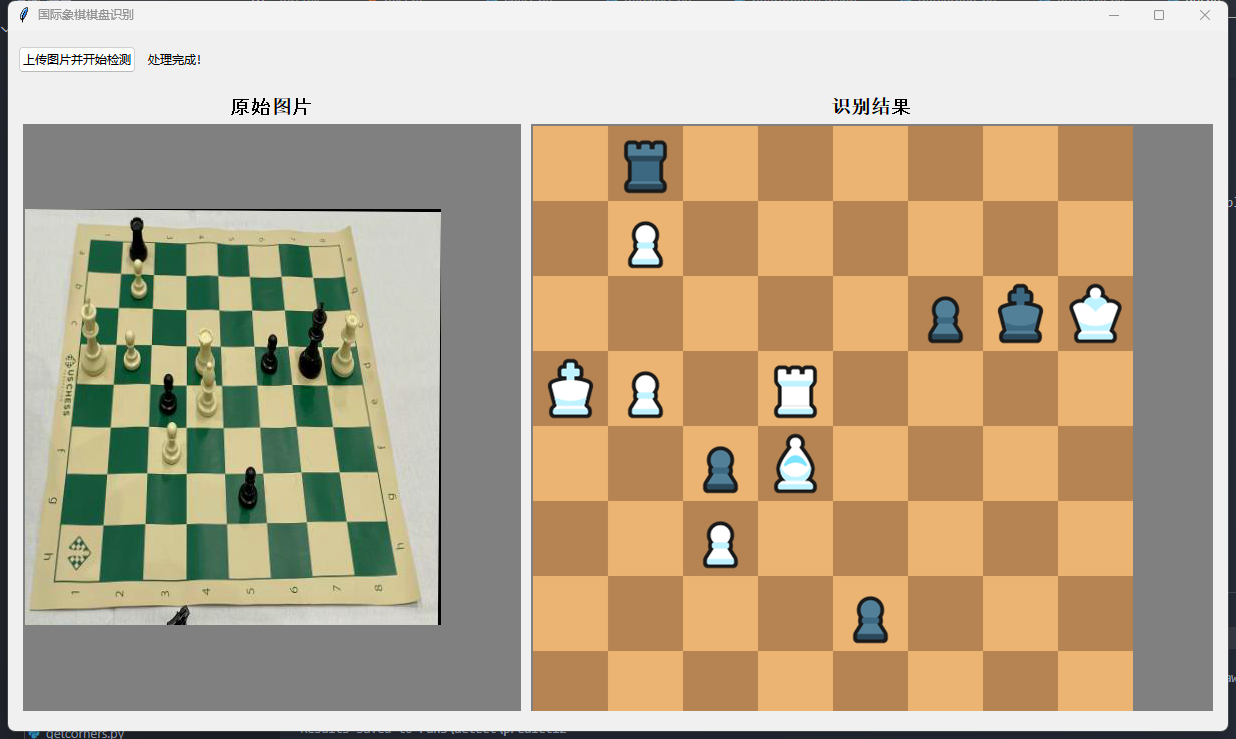
\includegraphics[width=0.9\textwidth]{image/gui.png} 
    \caption{系统图形用户界面 (GUI) 截图}
    \label{fig:gui}
\end{figure}

\subsection{工作流程}
当用户点击“上传图片并开始检测”按钮后,系统将执行以下一系列操作:
\begin{enumerate}
    \item 弹出文件选择对话框,让用户选择本地的棋盘图片。
    \item 加载并显示用户选择的原始图片到左侧区域。
    \item 调用后台核心处理逻辑,依次执行棋盘角点检测 (\texttt{getcorners.py}) 和棋子识别 (\texttt{getchess.py})。
    \item 将检测结果(角点坐标和棋子列表)进行透视变换和网格映射,重建出一个完整的\texttt{ChessBoard}对象。
    \item GUI前端根据\texttt{ChessBoard}对象的状态,使用预先加载的棋子图片资源(PNG格式),动态绘制出一个800x800像素的二维棋盘图像。
    \item 将最终生成的图像显示在右侧的结果区域,完成一次完整的识别过程。
\end{enumerate}
这种前后端分离的设计,使得用户无需关心复杂的后台处理细节,只需通过直观的界面即可与系统交互并获取最终结果。

\section{总结和讨论 (Discussion and Conclusions)}
本项目成功地开发了一个结合经典计算机视觉和深度学习的国际象棋识别系统。通过实验验证,该系统能够从单张图像中准确地提取棋盘布局,证明了所提方法的有效性。


\textbf{主要收获与思考}:
\begin{itemize}
    \item \textbf{混合方法的优势}:对于像棋盘这样具有强几何结构的对象,传统CV方法在定位和校正方面既高效又可靠。而对于形态多样、可能存在遮挡的棋子,深度学习模型则展现出无与伦比的识别能力。二者结合,相得益彰。
    \item \textbf{模块化设计的重要性}:将系统分解为棋盘定位、棋子检测和状态重建三个独立的模块,使得开发、调试和优化过程更加清晰和高效。每个模块都可以独立改进而不影响其他部分。
\end{itemize}

\textbf{局限性与未来工作}:
尽管系统表现良好,但仍存在一些可改进之处:
\begin{itemize}
    \item \textbf{角点检测的鲁棒性}:当前方法依赖于棋盘是图像中最大轮廓的假设,这在复杂背景下可能不成立。未来可以探索使用霍夫变换寻找棋盘网格线,或训练一个专门的CNN来直接回归角点位置,以提高鲁棒性。
    \item \textbf{棋子定位精度}:目前使用边界框的加权点来代表棋子位置,当棋子倾斜或边界框不紧密时可能产生偏差。更精确的方法是计算边界框底边中心点,或者使用实例分割模型(如\texttt{YOLOv11-seg})来获取棋子的掩码(\texttt{Mask}),从而计算其质心或底部中心,获得更精确的落点。
    \item \textbf{功能扩展}:当前系统仅处理静态图像。未来的工作可以将其扩展到视频流,通过跟踪棋子的移动来识别行棋步骤,甚至判断走法是否符合规则,从而实现一个完整的智能棋局分析系统。
\end{itemize}

% 若未使用BibTeX可保留如下手工文献列表
\begin{thebibliography}{9}
    \bibitem{yolo}
    Redmon, J., Divvala, S., Girshick, R., \& Farhadi, A. (2016). You Only Look Once: Unified, Real-Time Object Detection. In \textit{Proceedings of the IEEE conference on computer vision and pattern recognition (CVPR)}.
    
    \bibitem{opencv}
    Bradski, G. (2000). The OpenCV Library. \textit{Dr. Dobb's Journal of Software Tools}.
    
    % --- 修复:删除重复的条目 ---
    \bibitem{YOLOv11}
    Jocher, G., Chaurasia, A., \& Qiu, J. (2023). Ultralytics YOLOv11. \url{https://github.com/ultralytics/ultralytics}.
    
\end{thebibliography}

\end{document}